\documentclass[14pt]{extarticle}

%\usepackage[usenames,dvipsnames,svgnames,table]{xcolor}
\usepackage[a4paper,margin=15mm,lmargin=30mm]{geometry}

\usepackage{amsmath,amssymb,amsfonts}
\usepackage{mathtools}
\usepackage[cache=false,outputdir=.texpadtmp]{minted}

\usepackage{polyglossia}
\setmainlanguage{russian} 
\setotherlanguage{english}
\newfontfamily\russianfont[Script=Cyrillic]{CMU Serif}
\newfontfamily{\cyrillicfonttt}{CMU Typewriter Text}


%\newtheorem{definition}{Определение}
%\newtheorem{theorem}{Tеорема}

% Macro: Absolute value
\DeclarePairedDelimiter{\abs}{\lvert}{\rvert}

\begin{document}

%-----------------------------------------
% Титул
\thispagestyle{empty}

\begin{center}

\scriptsize{
Министерство образования и науки Российской Федерации

Федеральное государственное автономное образовательное учреждение высшего профессионального образования
}

\textbf{«Уральский федеральный университет}

\textbf{имени первого Президента России Б.Н. Ельцина»}

\textbf{\large Институт математики и компьютерных наук}

\textbf{\large Кафедра алгебры и дискретной математики}


\vfill
\vfill

\Large  О фильтрации событий в физике высоких энергий с помощью нейросетей с инверсией градиента.

\end{center}

%\end{onehalfspacing}
\vfill

\hspace*{0.4\textwidth}
\parbox{0.6\textwidth}{
\noindent
Квалификационная работа\\
на степень бакалавра наук\\
по направлению\\
«Математика, прикладная математика»\\
студента группы МТ-401\\
Киселева Антона Ивановича

\bigskip

\noindent
Научный руководитель\\
Клепинин Александр Владимирович,\\
кандидат физико-математических наук,\\
доцент кафедры алгебры и\\
дискретной математики ИМКН УрФУ
}

\vfill
\vfill

\begin{center}
Екатеринбург

2016
\end{center}

%\end{titlepage}
%-----------------------------------------

\sloppy

%-----------------------------------------
% Реферат
\newpage

\setcounter{page}{1}
\thispagestyle{empty}

\centerline{\large \textbf{Реферат}}

\bigskip
\bigskip

% TODO сократить
Глубокие нейросетевые архитектуры показывают превосходные результаты при наличии большого количества размеченных данных. В случае их отсутствия доменная адаптация помогает при наличии большого количества данных похожей природы, но имеющих смещенное распределение.
Одной из таких задач является фильтрация событий, полученных детекторами Большого Адронного коллайдера.
Для решения подобных задач была предложена новая архитектура для проведения доменной адаптации.
Ее суть заключается в создании нейросети с двумя выходами — один из них определяет класс, а другой домен.
Классифицирующие домен слои подключены к остальной сети при помощи слоя обращения градиента.
При проведении процедуры обучения при помощи метода обратного распространения ошибки этот слой негативно влияет на определение домена, таким образом нейросеть выделяет неспецифические для конкретных доменов признаки.

Целью этой работы является исследование применимости архитектуры нейросети со слоем обращения градиента в задаче детектирования распада частиц $\tau^- \rightarrow \mu^+ \mu^- \mu^-$.

В процессе работы была построена нейросеть, которая успешно обучается и выделяет признаки, позволяющие выделить сигнал, но не позволяющие по ним отделить реальные данные от синтетических.


\medskip

\noindent
Ключевые слова: доменная адаптация, глубокие нейронные сети.

\medskip 

\noindent
Объект исследования~— доменная адаптация глубоких нейронных сетей.

\medskip 

\noindent
Цель работы~— рассмотреть применение доменной адаптации нейронных сетей в задаче фильтрации событий, разработать методику применения таких сетей для создания неразличающего домены нейросетевого классификатора.

\medskip 

\noindent
Результаты работы: проведены эксперименты по применению данного вида нейросетей; изучено влияние изменения параметров классификатора на получаемый результат; сделан вывод насчет практической применимости доменной адаптации в данной задаче.

%-----------------------------------------
% Содержание
\newpage

\tableofcontents

%-----------------------------------------
% Введение
\newpage

\addtocontents{toc}{\protect{\contentsline{section}{\numberline{}{Введение}}{\thepage}}}
\section*{Введение}

% TODO редакция и расширение введения
Во многих задачах классификации применение глубоких нейронных сетей с архитектурой прямого распространения сигнала дает хорошие результаты. К сожалению, на данный момент эти задачи ограничиваются лишь такими, для которых имеется большое количество размеченных данных для обучения. В то же время, для некоторых задач с малым количеством размеченных данных возможно получить достаточный объем данных для обучения глубоких архитектур, которые распределение, смещенное относительно тестовых данных.
Важным примером таких задач являются задачи, для которых возможно получить множество размеченных синтетических данных, однако довольно часто их распределение будет отличным от реального. Обучение классификатора в условиях наличия смещения между тестовыми данными и данными для обучения называется доменной адаптацией.

В данной работе рассматривается предложенная в \cite{ganin} архитектура нейронной сети, позволяющая проводить доменную адаптацию.


%-------------------------------------------------------
% Теория
\newpage
\section{Теоретический материал}

В этой главе будет дано формальное определение задачи классификации, а так же будет описан один из методов ее решения — нейронная сеть.
% TODO ввод в главу

\subsection{Задача классификации}

Предполагаем, что модель получает на вход объекты $x \in X$, которым соответствуют метки классов $y \in Y$. Предполагается, что $Y = {1, 2, ..., L}$ — конечное множество размера $L$. $S(x,y), T(x,y)$ — распределения на $X \otimes Y$ будем называть \textit{исходным} и \textit{целевым} распределениями (или \textit{доменами}) соответственно. Далее считаем что между ними существует некоторый сдвиг — они в целом схожи, но различны.

Предполагаем, что нам даны ${x_1, x_2, ..., x_N}$ — обучающая выборка, выделенная как из исходного, так и из целевого доменов.
% TODO перефразировать выше, на самом деле там T(x), S(x) — marginal distribution

 Также нам известна бинарная переменная $d_i$, которая равна единице для объектов выборки из $S(x)$ и нулю для $T(x)$. Ее мы будем называть \textit{меткой домена}. При $d_i = 0$ нам известна метка класса $y_i$, иначе же нет. Именно ее нам необходимо предсказывать для тестовых данных.
 % TODO рерайт

\subsection{Устройство нейронной сети}

Нейронная сеть представляет собой сеть из нескольких слоев. У обычной нейронной сети есть по одному слою для входа и выхода. Также в обычной нейросети есть скрытые слои — они ими соединяются вход и выход. Они представляют собой матрицы весов. При работе нейросети она принимает некоторый вектор на вход, затем скрытые веса обрабатывают свои входы — умножают каждый из входов на его вес, затем все складывают и применяют активационную функцию. 
% TODO рерайт
% TODO использовать отсюда: http://neuralnetworksanddeeplearning.com/chap2.html

Для обучения нейросети чаще всего используется \textit{метод обратного распространения ошибки}. 

Так же для борьбы с переобучением между слоями нейросети вставляют dropout-слой. 
% TODO dropout + цитата

\subsection{Обучение нейронной сети}
% Этот раздел важен тем, что метод основывается на свойствах этого алгоритма обучения и работает (наверно) лишь только для него.
Приведем краткое описание используемого далее алгоритма обучения нейронной сети — стохастического градиентного спуска.
% TODO цитата + алгоритм

%-------------------------------------------------------
% Исследуемый метод
\newpage
\section{Исследуемый метод}
 
В этой главе мы опишем предложенную в \cite{ganin} архитектуру. Она представима в виде сети из трех отдельных сегментов.
 
Первый из сегментов будем называть \textit{экстрактором признаков} и обозначать $G_d$. Он занимается тем, что по исходному входу $x \in X$ возвращает вектор $f \in \mathbb{R}^D$. Если обозначить за $\theta_f$ параметры всех слоев экстрактора, то можно отметить что $f = G_d(x, \theta_d)$.
 
Второй сегмент $G_y$ затем продолжает первый и называется \textit{классификатором класса}. Он, очевидно, по выданным $G_f$ признакам $f$ возвращает метку $y$. Его параметры — $\theta_y$. Другими словами, $y = G_y(f, \theta_y)$.
 
Аналогично третий сегмент $G_d$ продолжает экстрактор признаков и возвращает метку домена $d$ и имеет параметры $\theta_d$: $d = G_d(f, \theta_d)$. Его называем \textit{классификатором домена}.
 
При проведении обучения нашей целью является получение признаков $f$, для которых распределения $S(f) = \{G_f(x; \theta_f)~|~x \sim S(x) \}$ и $T(f) = \{G_f(x; \theta_f)~|~x \sim T(x) \}$ будут схожи. Именно с этим и справляется предложенный в \cite{ganin} метод.

Метод рассматривает следующий функционал:

\begin{equation}\label{E}
\begin{gathered}
E(\theta_f, \theta_y, \theta_d) = \\ \sum_{ \substack{i=1..N \\ d_i=0} }L_y(G_y(G_f(x_i; \theta_i); \theta_y), y_i) - \lambda \sum_{ i=1..N } L_d(G_d(G_f(x_i; \theta_i); \theta_d), y_i) = \\\sum_{ \substack{i=1..N \\ d_i=0} } L_y^i(\theta_f, \theta_y) - \sum_{ i=1..N }  L_d^i(\theta_f, \theta_d)
\end{gathered}
\end{equation}
\begin{itemize}
\item $L_y(·, ·)$ —~ функция потерь классификатора класса;
\item $L_d(·, ·)$ —~ функция потерь классификатора домена;
\end{itemize}

Идея метода в следующем: классификатор домена подключается к экстрактору признаков через специальный \textit{слой обращения градиента}, описанный далее. Благодаря своим свойствам, он позволяет при проведении обучения получать такие параметры $\theta_f$, которые максимизируют функцию потерь классификатора домена, но при этом такие $\theta_d$, которые ее минимизируют.


%-------------------------------------------------------
% Задача
\newpage
\section{Задача}

Для исследования метода была выбрана задача из соревнования \cite{kaggle_contest} с сайта \texttt{kaggle.com}. Оно проходило с 20 июля по 12 октября 2015 года. Соревнующимся был дан набор данных, содержащий как синтетические, так и реальные данные из эксперимента LHCb Большого Адронного коллайдера. Было предложено по этим данным выявлять наличие событий, соответствующих распаду $\tau \rightarrow 3\mu$. Наблюдение таких событий означает нарушение предсказываемой Стандартной моделью симметрии.
% TODO больше физического бэкграунда?
Далее мы подробно опишем формат данных и использованные для ранжирования участников соревнования метрики.  

\subsection{Формат данных}
Для анализа участникам состязания были предоставлены четыре файла:
\begin{enumerate}
\item \texttt{training.csv} — набор размеченных данных для обучения классификатора, целевой переменной является переменная \texttt{signal}. Ее значение 1 описывает события сигнала, 0 — фона.
\item \texttt{check\_agreement.csv} — набор размеченных данных для проверки на согласованость (описана в \ref{agreement_metrics}). Признаки такие же, как и в \texttt{training.csv}, однако \texttt{signal} отвечает за домен — 1 для синтетических данных, 0 для реальных.
\item \texttt{check\_correlation.csv} — набор данных для проверки классификатора на коррелированность с массой. Включает дополнительный признак \texttt{mass}. Подробней описано в \ref{mass_metrics}.
\item \texttt{test.csv} — набор неразмеченных данных, для которых участникам необходимо предоставить метки классов.
\end{enumerate}
% TODO добавить все фичи

\subsection{Процедура проверки решения}

\label{agreement_metrics}
\subsubsection{Проверка на согласованность}
Так как для обучения классификатора участникам были предоставлены как реальные, так и синтетические данные, при создании хорошего классификатора возможно было бы использовать такие признаки, которые были плохо смоделированы для синтетических данных. 

Чтобы избежать этого, при проверке решения используется критерий Колмогорова-Смирнова. Он рассчитывается следующим образом:
\begin{equation*}
	KS = max \abs{F_{simulation} - F_{real}}
\end{equation*}
\begin{itemize}
	\item $F_{simulation}, F_{real}$ — функции распределения для синтетических и реальных данных соответственно
\end{itemize}
Для принятия проверочной системой решения требовалось, чтобы $KS < 0.09$.


\label{mass_metrics}
\subsubsection{Проверка на корреляцию с массой}
Помимо этого, полученный классификатор может в процессе обучения по предоставленным данным научиться восстанавливать массу исходной частицы, распад которой был зафиксирован. Такое поведение вызывает некорректную оценку фона и может привести к ложным обнаружениям сигнала.

Для проверки классификатора на корреляцию с массой исходной частицы применяется критерий Крамера-Мизеса. \cite{cramer} Для его вычисления функция распределения на всем диапазоне масс сравнивается с функцией распределения на некотором интервале. После этого итоговое значение для критерия усредняется по всем интервалам:
% TODO как точно называется критерий? цитата?

\begin{equation*}
	CvM_{interval} = \int (F_{global} - F_{local})^2 dF_{global},
\end{equation*}
\begin{equation*}
	CvM = <CvM_{interval}>_{interval}
\end{equation*}
\begin{itemize}
	\item $F_{global}, F_{local}$ — функции распределения для всех данных и для данных в некотором интервале масс
\end{itemize}
Чтобы решение засчитывалось, требовалось чтобы $CvM < 0.002$.

\subsubsection{Метрика качества}
Качество полученного классификатора оценивалось при помощи взвешенного показателя AUC. Этот показатель рассчитывается как площадь под ROC-кривой, построенной для результатов классификатора. В данном случае вклад в показатель AUC конкретных сегментов под ROC-кривой показан ниже:

\begin{center}
	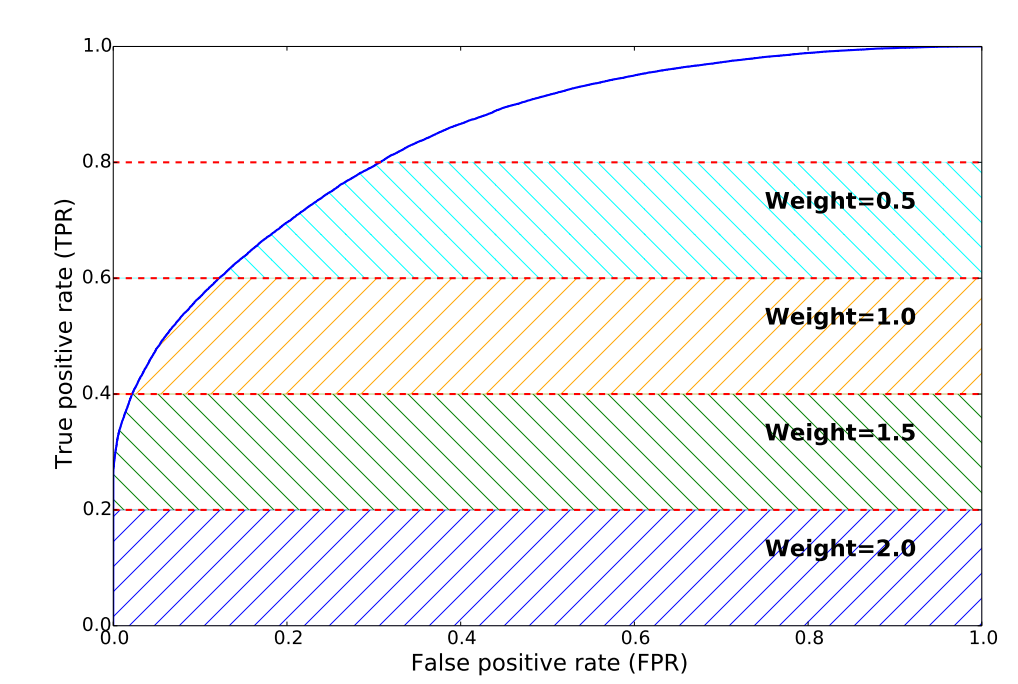
\includegraphics[scale=0.8]{auc.png}
\end{center}

%-------------------------------------------------------
% Применение метода к задаче
\newpage
\section{Применение метода к задаче}

%-------------------------------------------------------
% Описание использованной нейросетевой архитектуры
\subsection{Описание использованной нейросетевой архитектуры}

Для исследования метода было выбрано следующее строение: % TODO приложить картинку с наглядным описанием


Обучение происходит следующим образом.
Сначала нейросеть обучается при $\lambda = 0$ некоторое количество времени. После этого частично обученная сеть дает результат для данных соответствия, а затем дообучивается с их добавлением следующим образом: на вход классификатору домена для данных соотвествия выставляется метка, получанная ранее, а классификатору домена такая, которая уже находится в данных. Таким образом мы стараемся максимально сохранить результат именно классификатора класса, пытаясь изменить веса внутри экстрактора признаков. При этом мы плавно начинаем повышать $lambda$, каждый раз вычисляя метрики. Останавливаемся в тот момент, когда метрика KS не станет удовлетворять условиям соревнования, а именно станет меньше $0.09$. 

%-------------------------------------------------------
% Особенности программной реализации
\subsection{Особенности программной реализации}
Для решения задачи был выбран язык программирования Python, а так же фреймворк для проектирования нейронных сетей Keras. Выбор этих инструментов мотивирован простотой их использования.

% TODO научный стиль для всей сабсекции
Отметим отдельно особенности фреймворка Keras, позволяющие лучше описать нейросетевую модель. В версии 1.0.0 во фреймворке появилась так называемое Functional API. Продемонстрируем его применение:

\begin{minted}[fontsize=\small]{python}

n_extracted_features = 100
lam = 0.2

f = feature_extractor(input.shape[1], n_extracted_features)
l = label_classifier(n_extracted_features)
d = label_classifier(n_extracted_features,
                     name="domain_classifier")
	                     
model_input = Input(shape=(f[1],))
features = f(model_input)
label_class = l(features)
grl = GradientReversal(lam, 
                input_shape=(domain_classifier.input_shape[1],))
domain_class = d(grl(f))
m = Model(input=[model_input], output=[label_class, domain_class])
m.compile(loss=['categorical_crossentropy',
   'categorical_crossentropy'], loss_weights=[1, 1],
   metrics=['accuracy', 'accuracy'], optimizer='rmsprop') 
\end{minted}

Как можно заметить, вместо описывания в коде нейросети графом, расписывая всех слоев и всех связей между ними, нам требуется лишь передать каждому следующему слою предыдущий, как будто следующий слой является функцией предыдущего. Именно по этому этот API и имеет такое название.

%-------------------------------------------------------
% Методика проверки работы метода
\subsection{Методика проверки работы метода}

% TODO как оцениваем полученные решения?


%-----------------------------------------
% Результаты проверки
\newpage
\section{Результаты проверки}

% TODO can i haz pikz?
В результате можно заметить, что в самом начале нейронная сеть обучается одинаково как на одном выходе, так и на другом. Однако с увеличением параметра $\lambda$ и добавлением проверочных данных, метрика KS начинает снижаться до требуемого условиями состязания уровня и дальше. Однако с этим процессом так же падает и метрика AUC, а с ней и место в рейтинге на Kaggle. Помимо этого, при дальнейшем обучении нейросеть переобучается, что выливается в нестабильное поведение метрики KS и сильном увеличении метрики CvM, а так же в падение качества на валидации. 

Метод показал свою работоспособность в этой задаче, однако его все еще можно улучшить. Некоторые из таких способов: после выделения признаков можно попробовать использовать другие методы машинного обучения, вроде градиентного бустинга; можно получить больше данных, а именно применение синтетических данных из другого домена может улучшить выделение признаков. Помимо этого, метод стоит попробовать в других задачах.
% TODO рерайт, больше?

%-----------------------------------------
% Заключение
\newpage
\section*{Заключение}
\addtocontents{toc}{\protect{\contentsline{section}{\numberline{}{Заключение}}{\thepage}}}

В работе продемонстрировано применение доменной адаптации в задаче фильтрации событий для детектора частиц коллаборации LHCb Большого Адронного Коллайдера. Были рассмотрены различные приемы обучения нейросетевого классификатора. В результате было получено решение задачи Flavours of Physics на сайте Kaggle, показывающее результат лучше методов, используемых в ЦЕРН. 

Полученную нейронную сеть возможно с легкостью адаптировать для решения других задач.
% TODO подробней

%-----------------------------------------
% Литература
\newpage
\addtocontents{toc}{\protect{\contentsline{section}{\numberline{}{Список литературы}}{\thepage}}}

\begin{thebibliography}{3}  

\bibitem{ganin}
\textit{Yaroslav Ganin, Victor Lempitsky.} Unsupervised Domain Adaptation by Backpropagation \\ \texttt{http://arxiv.org/pdf/1409.7495.pdf}

\bibitem{keras}
\textit{François Chollet.} keras, репозиторий GitHub \\ \texttt{https://github.com/fchollet/keras}

\bibitem{kaggle}
\textit{Thomas Blake, Marc-Olivier Bettler, Marcin Chrząszcz, Francesco Dettori, Andrey Ustyuzhanin, Tatiana Likhomanenko.} Flavours of Physics: the machine learning challenge for the search of $\tau^-\rightarrow\mu^+ \mu^- \mu^-$ decays at LHCb \\ \texttt{
	https://kaggle2.blob.core.windows.net/competitions/kaggle/\\4488/media/lhcb\_description\_official.pdf
	}
	
\bibitem{kaggle_contest}
 Flavours of Physics: Finding $\tau^-\rightarrow\mu^+ \mu^- \mu^-$ \\ \texttt{https://www.kaggle.com/c/flavours-of-physics/}

\bibitem{cramer}
H. Cram\'er. On the composition of elementary errors — Scandinavian Actuarial Journal, 1928 % http://www.tandfonline.com/doi/pdf/10.1080/03461238.1928.10416862

\end{thebibliography}

\label{page:last}

\end{document}
